\section{Empirical Evaluation}
In this section, we make an empirical evaluation of our algorithm by performing a set of experiments on the synthetic data set, and several real world data sets.

\subsection{Comparison Methods}
In order to evaluate the effectiveness of our algorithm, we choose three time series similarity algorithms and four correlation coefficient in our experiment. 

For the three similarity algorithm, we choose L1-Distance, L2-Distance \cite{han2011data}, and DTW-Distance \cite{muller2007dynamic}. 
And for the three similarity algorithm, we choose Pearson correlation \cite{nagelkerke1991note}, which is the widely used methods for correlation mining in time series. And also two ranking based correlation: The Kendall rank correlation \cite{kendall1938new}, and Spearman's rank correlation \cite{pirie1988spearman}.

In the rest of this subsection, we briefly introduce the three similarity measures and the three Correlation measures.
 
\subsubsection{Similarity Measures}

Given a two time series 
$X=(x_1,x_2,...,x_m),Y=(y_1,y_2,...,y_m)$.

The L1-distance is denoted as follow:

\begin{equation}
L1(X,Y) = \sum_{1}^{m}|x_i-y_i|
\end{equation}

The L2-distance is denoted as follow:

\begin{equation}
L1(X,Y) = \sqrt{\sum_{1}^{m}|x_i-y_i|^2}
\end{equation}

The third similarity measure we used is DTW distance \cite{muller2007dynamic}, which is a famous time series similarity measure.

In order to introduce the DTW distance, we firstly construct an $m-by-m$ matrix $W$, where the $(i-{th},j-{th})$ element of the matrix $W$. The DTW distance is to find a path through the matrix that minimizes the total cumulative distance between $X$ and $Y$. 
So, the optimal path is the path that minimize the warping cost:

\begin{equation}
DTW(X,Y) = \min { \sqrt{\sum_{k=1}^{K}w_k}}
\end{equation}
where, $w_k$ belongs to the $k-{th}$ element of a warping path $P$, which is a contiguous set of elements that represent a mapping between $X$ and $Y$.

\subsubsection{Correlation Measures}

In this subsection, we introduce three widely used correlation measures between time series: Pearson Correlation \cite{pearson1904mathematical}, Kendall rank correlation \cite{kendall1938new}, and Spearman's rank correlation \cite{pirie1988spearman}.

The Pearson correlation method is one of the most widely used method for measuring the correlation between two time series. The Pearson correlation coefficient, denoted as $\rho$. can be calculated as follow:

\begin{equation*}
\rho_{X,Y}^{Pearson}=\frac{cov(X,Y)}{\sigma_X\sigma_Y}=\frac{E[(X-\mu_X)(Y-\mu_Y)]}{\sigma_X\sigma_Y}
\end{equation*}
where $cov$ is the covariance, $\sigma_X$ is the standard deviation of $X$, $\mu_X$ is the mean of $X$ and $E[*]$ denotes the expectation.

The Kendall rank correlation \cite{kendall1938new} is defined as follow:

\begin{equation*}
\rho_{X,Y}^{Kendall}=\frac{N_c - N_d}{m(m-1)/2}
\end{equation*}

Where $N_c$ is the number of concordant pairs, and $N_d$ is the number of discordant pairs, and $m$ is the dimension of the time series.
For any pair $(x_i,y_i)$ and $x_j,y_j$, where $i \neq j$, are said to be concordant both $x_i > x_j$ and $y_i > y_j$, or $x_i < x_j$ and $y_i < y_j$. Otherwise, they are discordant.

The Spearman's rank correlation \cite{pirie1988spearman} is defined as follow:

\begin{equation*}
\rho_{X,Y}^{Spearman}=1 - \frac{6\sum d^2_i}{n(n^2-1)}
\end{equation*}

where $d_i$ is defined as the difference between the ranks of $x_i$ and $y_i$.

\subsection{Effectiveness Study on Synthetic Dataset}

In this section, we introduce the experiment on the synthetic Dataset.

\subsubsection{The Synthetic Dataset}

Synthetic data set is very useful for evaluating algorithms and functions for data mining and machine learning models\cite{han2011data}. 
In this section, we introduce the Synthetic Dataset used in our experiment.

In this synthetic Dataset, we randomly generate $10000$ time series with two patterns of time series: (1) Periodical Pattern, (2) Linear Pattern.
Each time series was added with white noise \cite{han2011data}. 
Then, we separate the $10000$ time series into five groups. And within each group, we add change randomly at the same time. (In each group, the change points are same.)
Seven different types of changes are added randomly into each time series, the seven change types are showed in Table.\ref{Tab:ChangeType}.

\begin{table}[t]
\caption{\textbf{Change Types in the Synthetic Data}}
\centering

\begin{tabular}{|c|}
\hline Change Type \\
\hline Mean Change \\
\hline Variance Change\\
\hline Frequency Change $+$ Variance Change\\
\hline Mean Change $+$ Frequency Change \\
\hline Frequency Change $+$ Variance Change\\
\hline Mean Change $+$ Frequency Change $+$ Variance Change\\
\hline
\end{tabular}
\label{Tab:ChangeType}
\end{table}

In order to test both the efficiency and effectiveness of change based correlation coefficient. We choose four sub-set from such dataset. 
We make the data set size from small to large, and also the time series length from short to long. The four sub dataset is showed in Table.\ref{Tab:SDataScale}. 

\begin{table*}
\caption{Clustering Performance on Synthetic Data Set}
\centering
\renewcommand{\arraystretch}{1.2}
\begin{tabular}{ccccccccc} 
\toprule[2pt] 
%\hline
Dataset & Measure & Proposed & $L1$ & $L2$ & DTW & Pearson & Kendall & Spearman \\
\toprule[1.5pt] 
\multirow{2}*{\centering{Sythetic-T0}}
     & Accuracy & $\boldsymbol{.854\pm.032}$ & $.241\pm.098$ & $.281\pm.012$ & $.230\pm.061$ & $.309\pm.140$ & $.353\pm.026$ & $.297\pm.036$ \\
\cline{2-9}
     & NMI & $\boldsymbol{.808\pm.034}$ & $.026\pm.067$ & $.076\pm.023$ & $.028\pm.075$ & $.140\pm.55$ & $.395\pm.015$ & $.150\pm.088$ \\
\toprule[1.2pt] 
\multirow{2}*{\centering{Sythetic-T1}}
     & Accuracy & $\boldsymbol{.838\pm.025}$ & $.247\pm.026$ & $.262\pm.032$ & $.283\pm.012$ & $.240\pm.018$ & $.374\pm.067$ & $.341\pm.067$ \\
\cline{2-9}
     & NMI & $\boldsymbol{.701\pm.030}$ & $.003\pm.062$ & $.057\pm.043$ & $.064\pm.036$ & $.046\pm.084$ & $.404\pm.023$ & $.230\pm.042$ \\
\toprule[1.2pt] 
\multirow{2}*{\centering{Sythetic-T2}}
     & Accuracy & $\boldsymbol{.806\pm.029}$ & $.254\pm.066$ & $.263\pm.080$ & $.304\pm.022$ & $.388\pm.024$ & $.384\pm.032$ & $.502\pm.182$ \\
\cline{2-9}
     & NMI & $\boldsymbol{.889\pm.012}$ & $.028\pm.042$ & $.056\pm.056$ & $.054\pm.032$ & $.303\pm.064$ & $.394\pm.052$ & $.450\pm.049$ \\
\toprule[1.2pt] 
\multirow{2}*{\centering{Sythetic-T3}}
     & Accuracy & $\boldsymbol{.856\pm.077}$ & $.225\pm.028$ & $.229\pm.034$ & $.284\pm.062$ & $.454\pm.032$ & $.454\pm.032$ & $.454\pm.032$ \\
\cline{2-9}
     & NMI & $\boldsymbol{.891\pm.017}$ & $.021\pm.040$ & $.041\pm.043$ & $.086\pm.038$ & $.454\pm.032$ & $.454\pm.032$ & $.454\pm.032$ \\
\bottomrule[1.5pt] 
\end{tabular}
\label{Tab:ClusRes}
\end{table*}


\begin{table}[t]
\caption{Summery of Synthetic Data}
\centering

\begin{tabular}{|c|c|c|}
\hline DataSet &  Data Size & Time Series Length\\
\hline Synthetic-T0 & 1000 & 800 \\
\hline Synthetic-T1 & 1000 & 5000 \\
\hline Synthetic-T2 & 10000 & 800 \\
\hline Synthetic-T3 & 10000 & 5000 \\
\hline
\end{tabular}
\label{Tab:SDataScale}
\end{table}

\begin{figure*}[t]
\centering
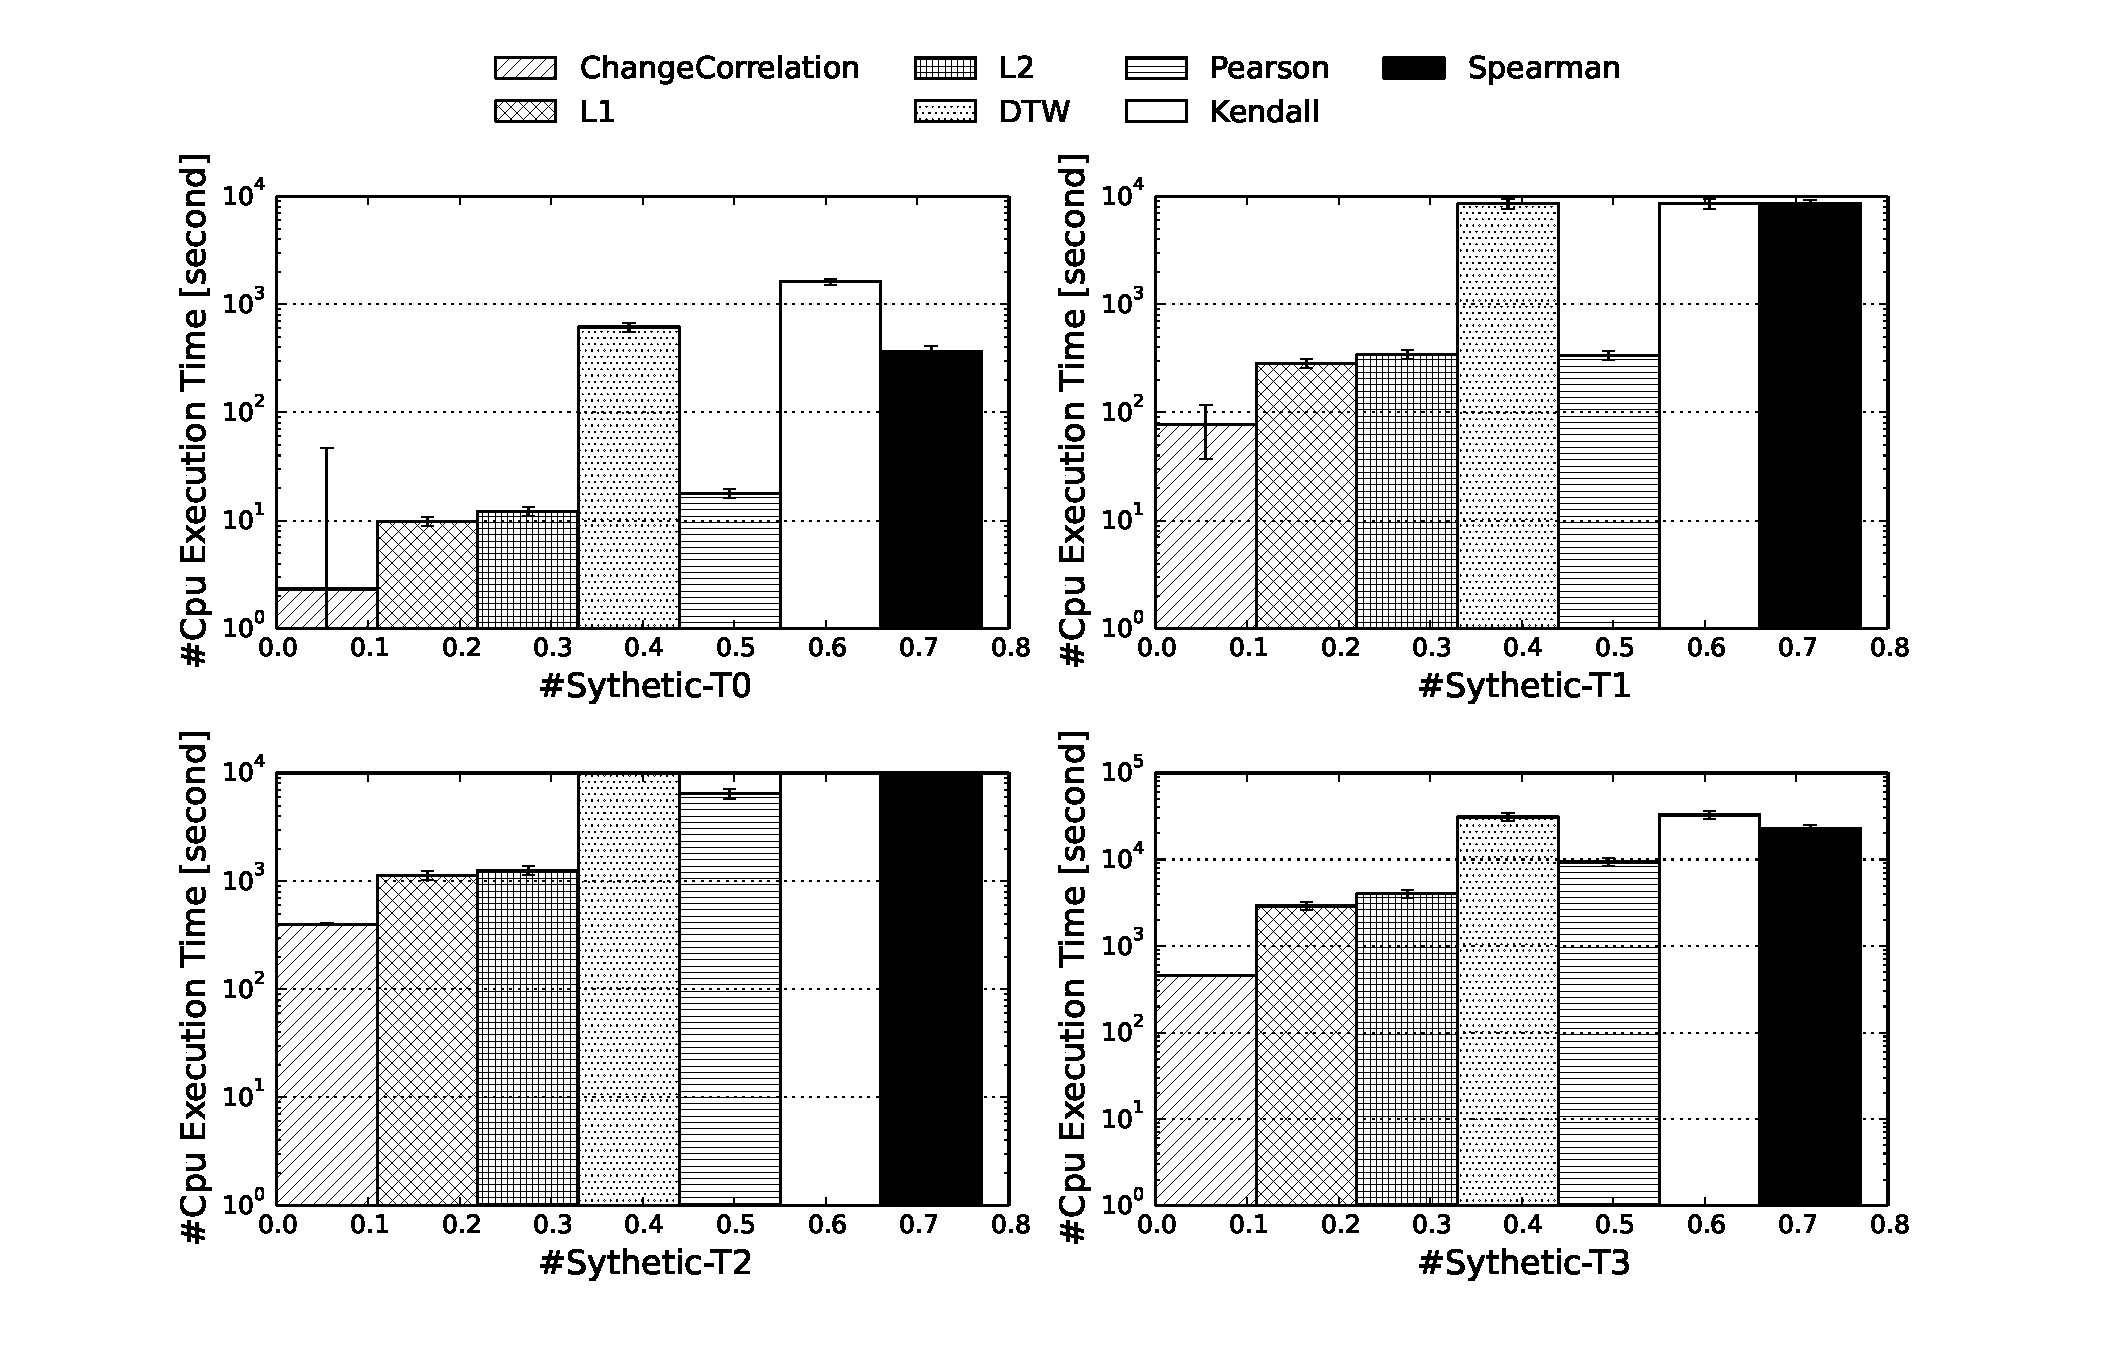
\includegraphics[width=0.8\textwidth]{SythClusPerf.eps}
\caption{Top-k Nearest Neighbor Search}
\label{Fig:ClusPerf}
\end{figure*}

\begin{figure*}[t]
\centering

\subfigure{%
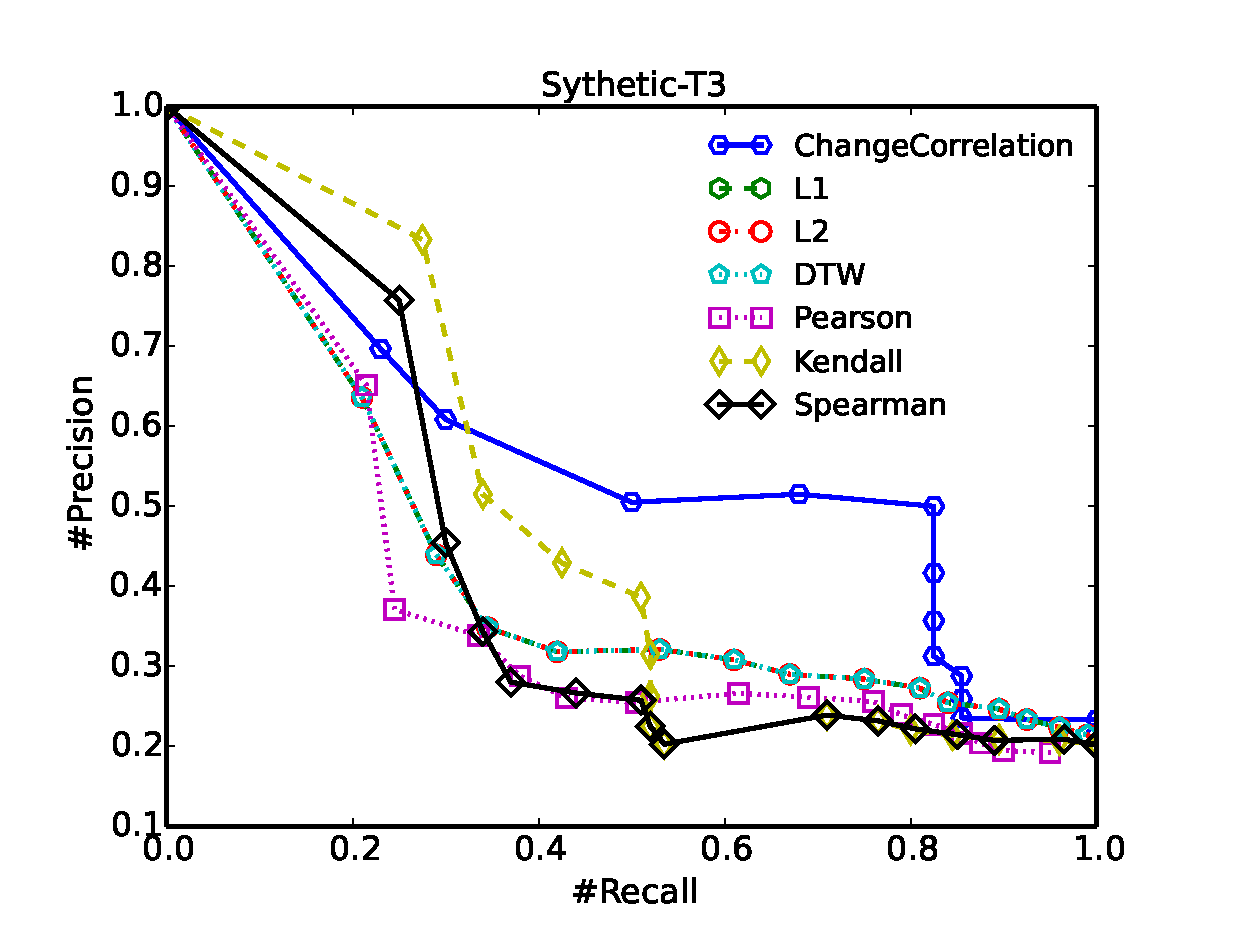
\includegraphics[width=0.41\textwidth]{PRC3.eps}
}\hspace{0.001em}
\subfigure{%
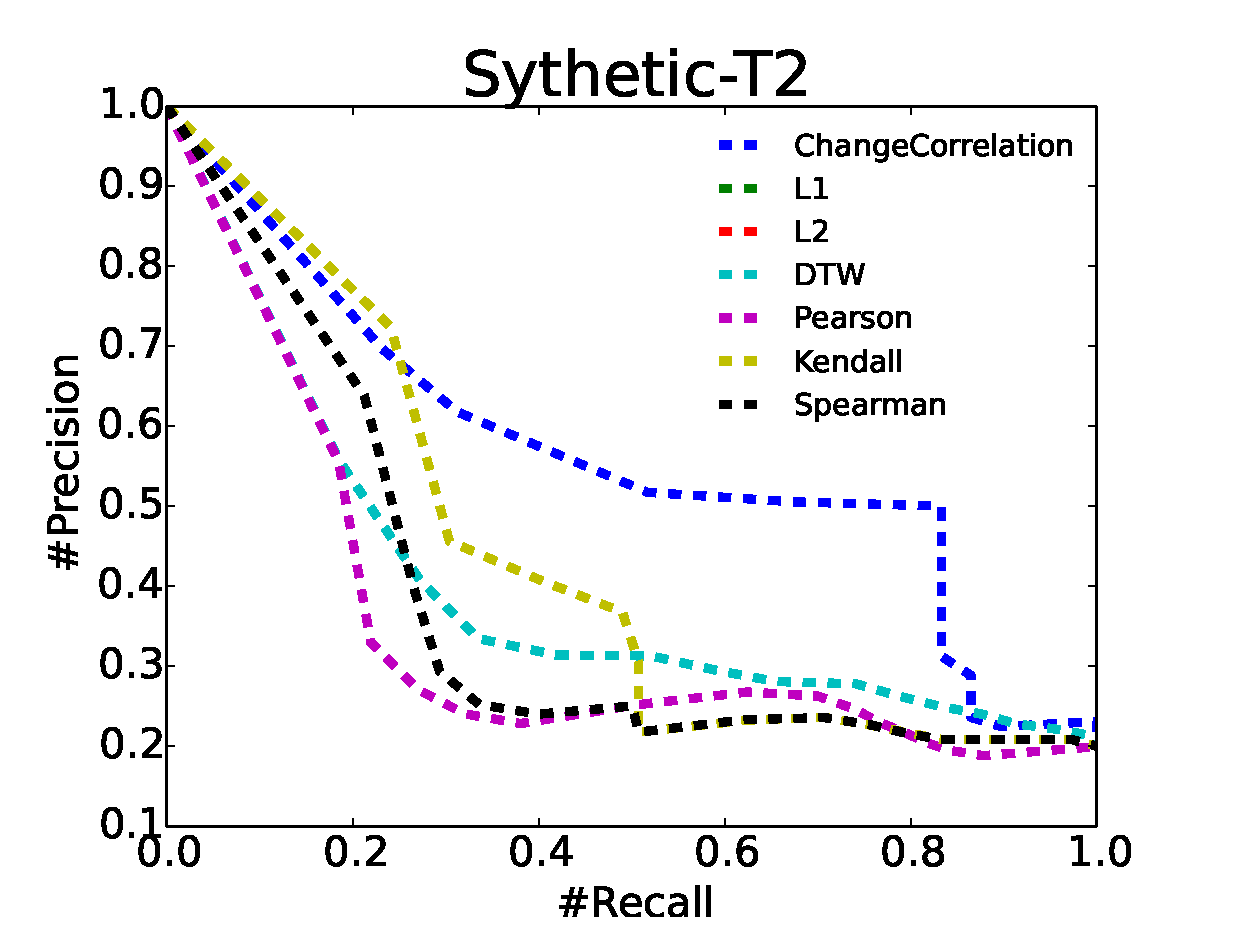
\includegraphics[width=0.41\textwidth]{PRC2.eps}
}\hspace{0.001em}
\subfigure{%
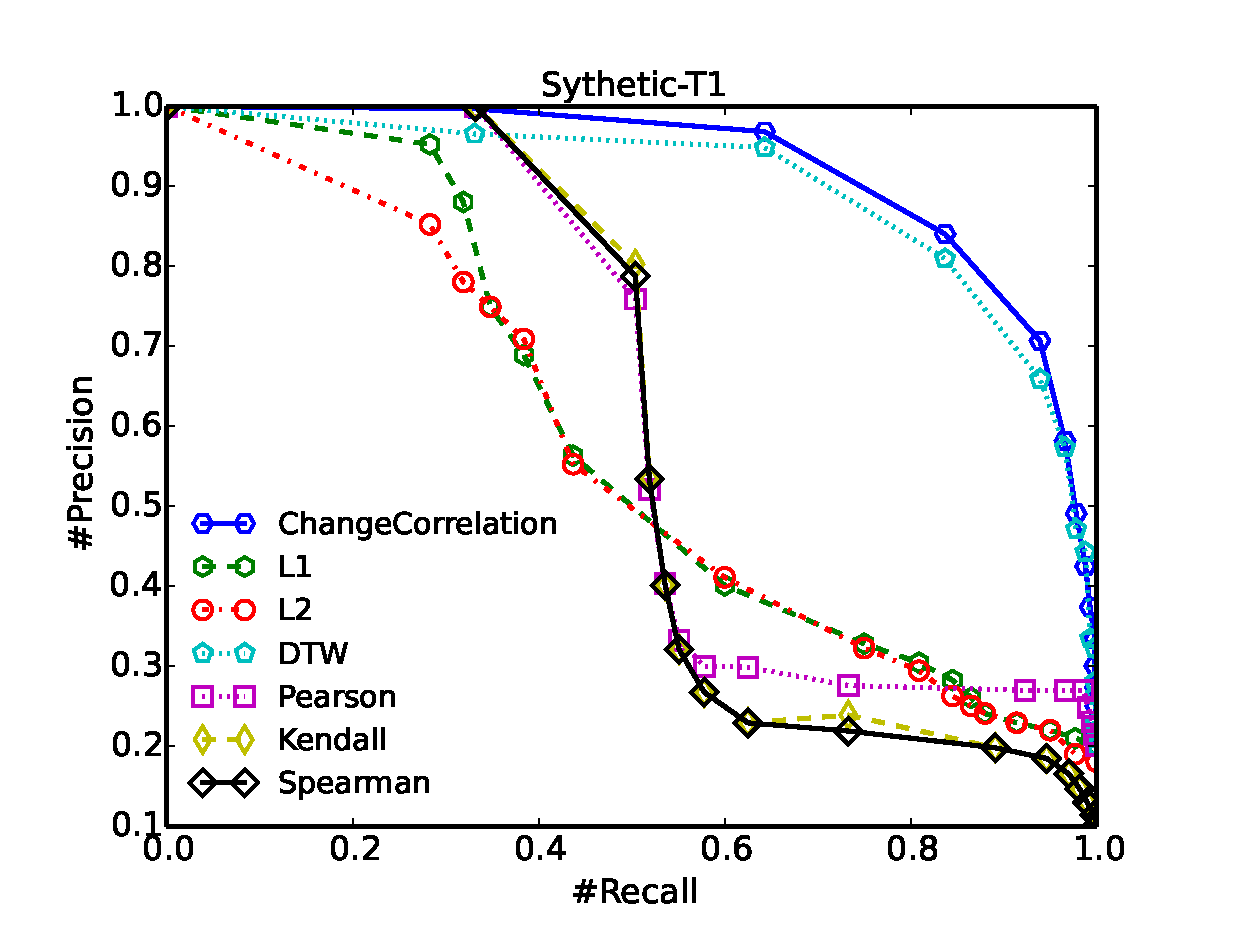
\includegraphics[width=0.41\textwidth]{PRC1.eps}
}\hspace{0.001em}
\subfigure{%
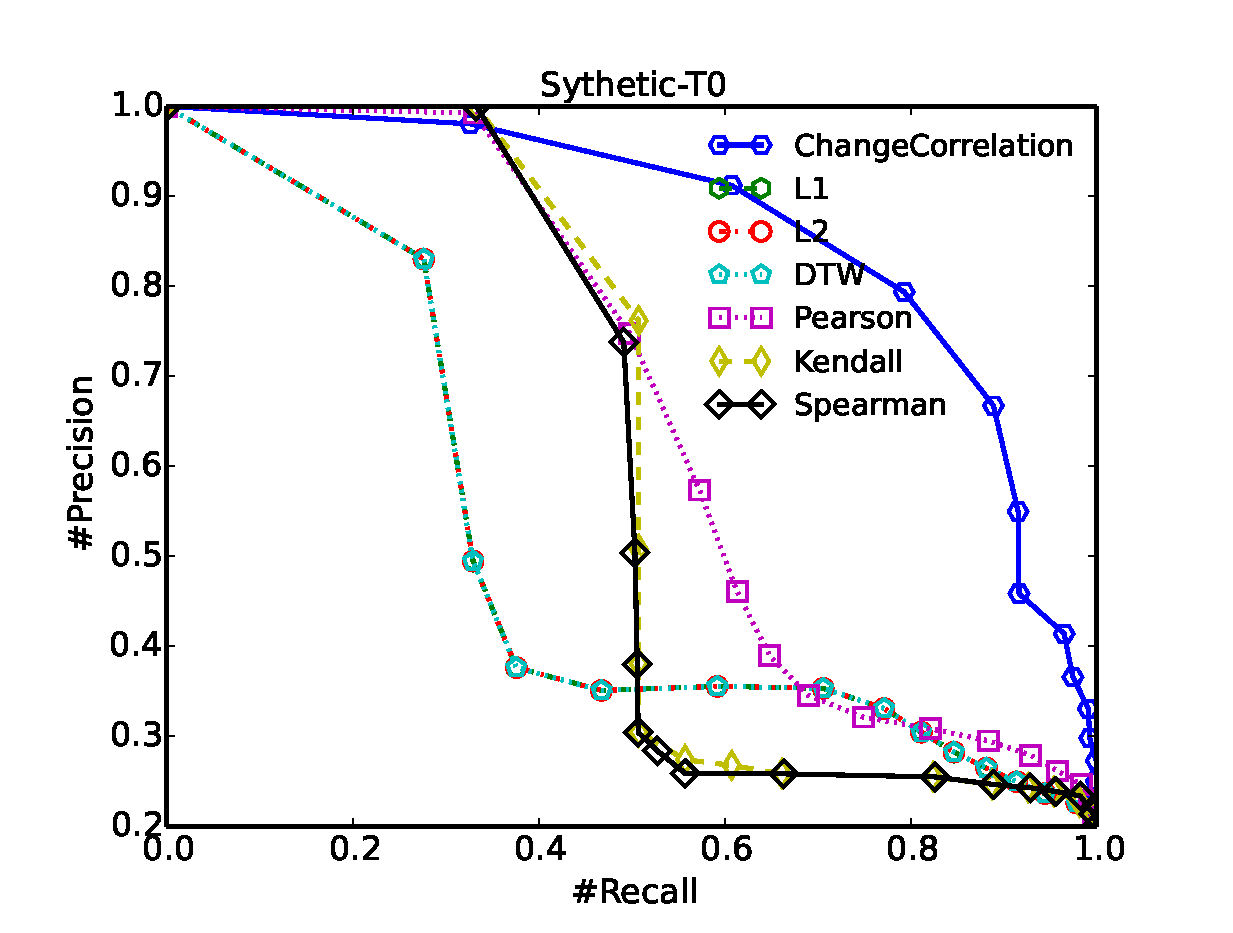
\includegraphics[width=0.41\textwidth]{PRC0.eps}
}
%
\caption{Precision Recall Curve for Different Algorithms}
\label{fig:NNPreRe}
\end{figure*}


\begin{figure*}
\centering
\subfigure{%
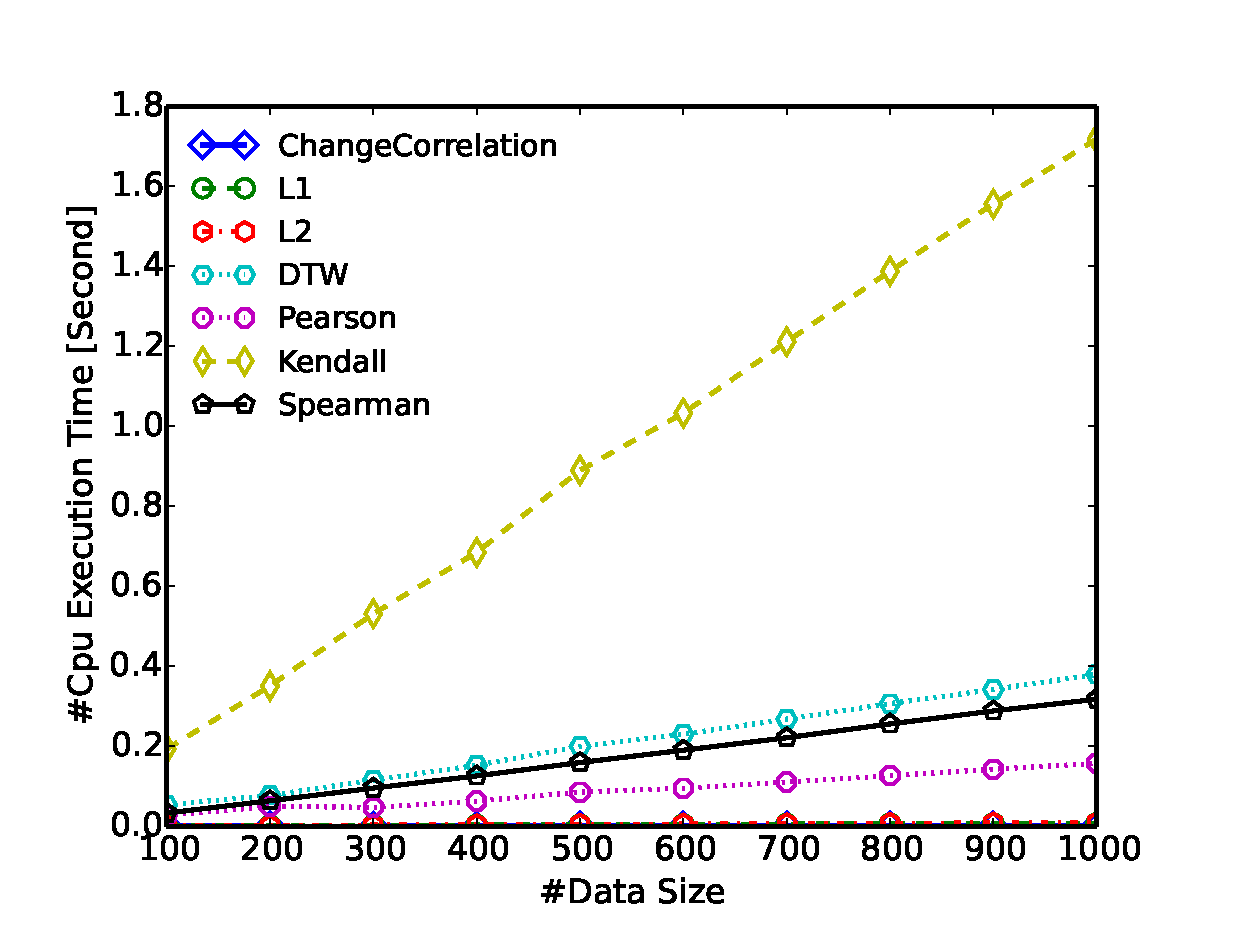
\includegraphics[width=0.45\textwidth]{VaryDataSize.eps}
}\hspace{0.001em}
\subfigure{%
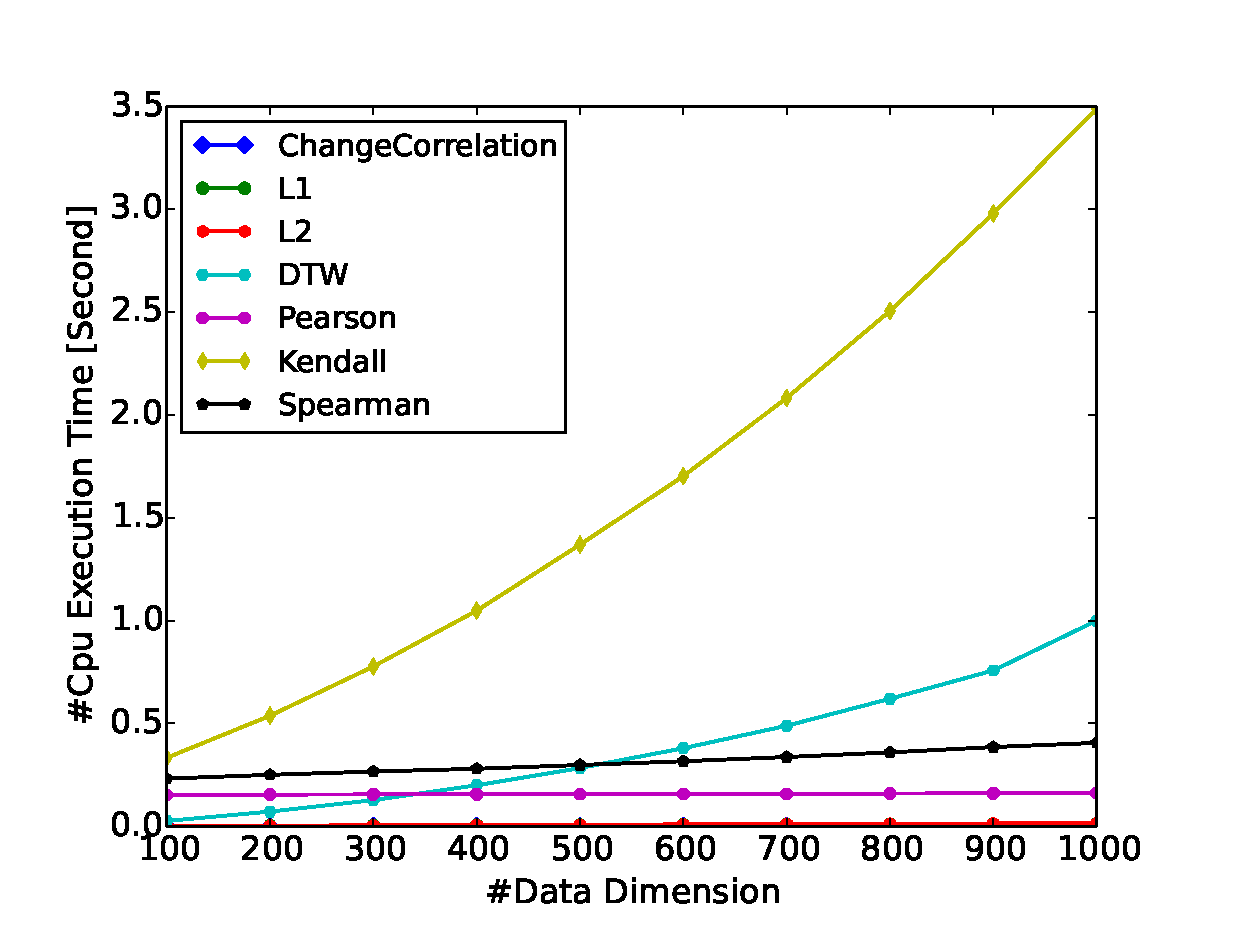
\includegraphics[width=0.45\textwidth]{VaryDataDimension.eps}
}\hspace{0.001em}
\caption{Efficiency by varying data size and dimension size}
\label{fig:NNPerf}
\end{figure*}


\subsubsection{Clustering Task}

In order to evaluate the performance of our correlation coefficient, we design a clustering task on the Synthetic Time series data. In this experiment, we only use the Hierarchical Clustering \cite{han2011data} to evaluate the performance. Because Hierarchical Clustering is very sensitive to the distance measure used, it is good for evaluating the distance measure.

Two evaluation methods are used for testing the clustering result: Accuracy \cite{han2011data}, which is calculated as the percentage of target objects clustered into the correct clusters; and Normalized Mutual Information (NMI) \cite{han2011data}, which is one of the most popular evaluation methods to evaluate the quality of clustering results.

From Table.\ref{Tab:ClusRes}, we can see that, for the change correlation coefficient, the clustering result performance is better for the high dimensional data set.
This is because that for high dimensional time series data, the proposed coefficient can extract more change information from the time series data and also make more accurate evaluation of the correlation. 
From this point of view, change based correlation is more suitable for the high dimensional time series data set.
On the other hand, Change based correlation can obtain more accuracy results in different dataset compared with both the similarity method and the correlation coefficient. So, the result of clustering show the effectiveness of our coefficient.

Fig.\ref{Fig:ClusPerf} shows the Execution time of the clustering task on each data set. From the result, we can see that change based correlation performed much faster than other algorithms. This is because, we only calculate the correlation on the extracted change information (Bit-stream), the calculating of change based correlation measure can be much faster than other similarity and correlation methods.


\subsubsection{Top-K Searching Task}

We compute precision and recall \cite{powers2011evaluation} on the data-set using the LSH-based method. And for other distance measure, we use the naive Top-K searching method. 

For precision and recall, if the Searched time series is in the same cluster of the query time series, we regard it as a relevant items, and vice verse. We range the $K$ from $1$ to the cluster size. 

For each top-k Nearest Neighbors search, the precision can be calculated as follow:

\begin{equation}
Precision =\frac{relevant~item}{K} 
\end{equation}

and the recall can be calculated as follow:

\begin{equation}
Precision =\frac{relevant~item}{Relevant~Cluster~Size} 
\end{equation}

The plots for all the three datasets are shown in Figure.\ref{fig:NNPreRe}.
We can clearly see that our proposed Change-based Correlation method gives significantly higher precision recall curves than other similarity and correlation methods. In addition the results are consistent across datasets.

Fig.\ref{fig:NNPerf} shows the execution time by vary the data size and the time series length.
In left one of Fig.\ref{fig:NNPerf}, we fix the value of time series length, and
vary the data size n. We can see that the CPU execution
time of other similarity methods increased sharply by enlarging the data size. 
And, the change based correlation do not change so much by enlarge the data size.

In right of Fig. \ref{fig:NNPerf}, we fix the size of data size, and vary the value of time series length. Based on the results, we can see that the running time of the proposed change based method with LSH doesn't so much with the increase of time series length, while other methods increase by enlarging the time series length.

\subsection{Effectiveness Study on Real Datasets}

In this section, we will compare the proposed algorithm with the baseline algorithms on two real data sets.

\subsubsection{Electrocardiogram Data set}

The first real world dataset is ECG (Electrocardiogram) time series data set. This data set comes from the the UCR time series Data set Archive \cite{UCRArchive}. We choose four ECG data set there as showed in Table. \ref{Tab:ECGData}. And the ground truth comes from the UCR data set itself.

For the clustering task, we use the Hierarchical Clustering \cite{han2011data} to evaluate the performance as before. 
From Table.\ref{Tab:ECGClus}, we can see that, for the change based correlation can obtain more accuracy results in these four ECG data set compared with both the similarity method and the correlation coefficient. So, the result of clustering show the effectiveness of our coefficient.

For the Top-K searching task. The plots for all the four ECG dataset datasets are shown in Figure.\ref{fig:ECGPRC}.
We can clearly see that our proposed Change-based Correlation method gives significantly higher precision recall curves than other similarity and correlation methods. In addition the results are consistent across datasets. This demonstrate the effectiveness of change-based correlation coefficient and the corresponding LSH search algorithm.

\begin{table*}[t]
\caption{Summary of the Four ECG Data Set}
\centering

\begin{tabular}{|c|c|c|c|}
\hline Data Set & \centering Data Size & Time Series Length & Class Numver\\
\hline CinC_ECG_torso & \centering 1380 & 1639 & 4\\
\hline ECGFiveDays & \centering 861 & 136 & 2\\
\hline TwoLeadECG & \centering 1139 & 82 & 2\\
\hline ECG5000 & \centering 4500 & 140 & 5\\
\hline
\end{tabular}
\label{Tab:ECGData}
\end{table*}

\begin{table*}[t]
\caption{Clustering Performance on Synthetic ECG Data Set From UCR Time Series Archive}
\centering
\renewcommand{\arraystretch}{1.2}
\begin{tabular}{ccccccccc} 
\toprule[2pt] 
%\hline
Dataset & Measure & Proposed & $L1$ & $L2$ & DTW & Pearson & Kendall & Spearman \\
\toprule[1.5pt] 
\multirow{2}*{\centering{CinC_ECG_torso}}
     & Accuracy & $\boldsymbol{.839\pm.011}$ & $.667\pm.068$ & $.557\pm.012$ & $.610\pm.061$ & $.531\pm.140$ & $.507\pm.019$ & $.504\pm.013$ \\
\cline{2-9}
     & NMI & $\boldsymbol{.489\pm.019}$ & $.236\pm.035$ & $.019\pm.023$ & $.010\pm.075$ & $.280\pm.55$ & $.150\pm.015$ & $.049\pm.012$ \\
\toprule[1.2pt] 
\multirow{2}*{\centering{EGG_5000}}
     & Accuracy & $\boldsymbol{.538\pm.025}$ & $.247\pm.026$ & $.262\pm.032$ & $.283\pm.012$ & $.240\pm.018$ & $.374\pm.067$ & $.341\pm.067$ \\
\cline{2-9}
     & NMI & $\boldsymbol{.401\pm.030}$ & $.003\pm.062$ & $.057\pm.043$ & $.064\pm.036$ & $.046\pm.084$ & $.404\pm.023$ & $.230\pm.042$ \\
\toprule[1.2pt] 
\multirow{2}*{\centering{TwoLeadECG}}
     & Accuracy & $\boldsymbol{.810\pm.029}$ & $.504\pm.066$ & $.538\pm.080$ & $.620\pm.022$ & $.528\pm.064$ & $.531\pm.052$ & $.519\pm.049$ \\
\cline{2-9}
     & NMI & $\boldsymbol{.680\pm.012}$ & $.081\pm.042$ & $.043\pm.056$ & $.137\pm.032$ & $.047\pm.064$ & $.062\pm.052$ & $.074\pm.049$ \\
\toprule[1.2pt] 
\multirow{2}*{\centering{ECGFiveDays}}
     & Accuracy & $\boldsymbol{.832\pm.077}$ & $.502\pm.028$ & $.527\pm.034$ & $.615\pm.062$ & $.506\pm.032$ & $.547\pm.032$ & $.519\pm.032$ \\
\cline{2-9}
     & NMI & $\boldsymbol{.765\pm.017}$ & $.002\pm.040$ & $.002\pm.043$ & $.361\pm.038$ & $.075\pm.032$ & $.023\pm.032$ & $.086\pm.032$ \\
\bottomrule[1.5pt] 
\end{tabular}
\label{Tab:ECGClus}
\end{table*}

\begin{figure*}[t]
\centering
\subfigure{%
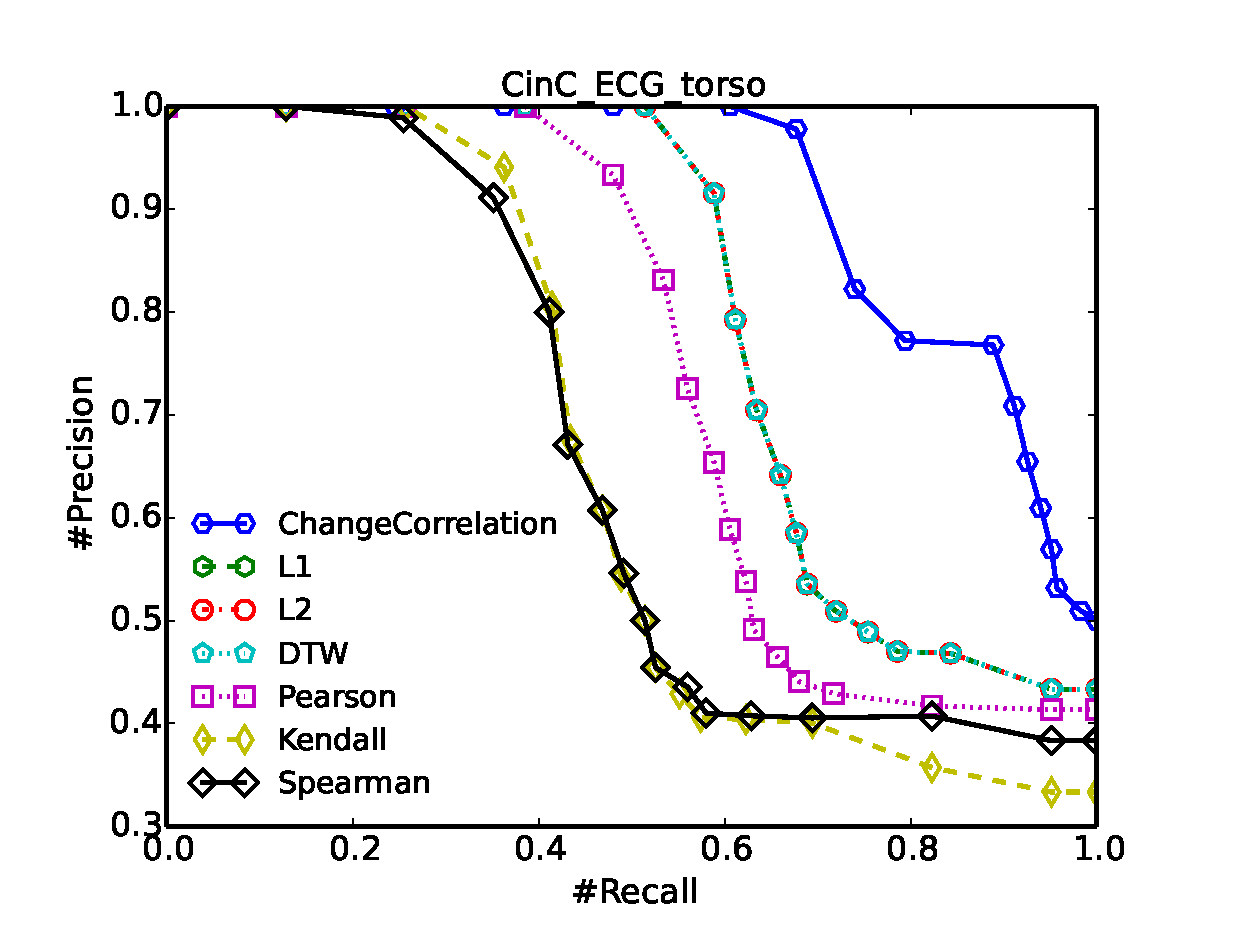
\includegraphics[width=0.45\textwidth]{PRCCinCECGtorso.eps}
}\hspace{0.001em}
\subfigure{%
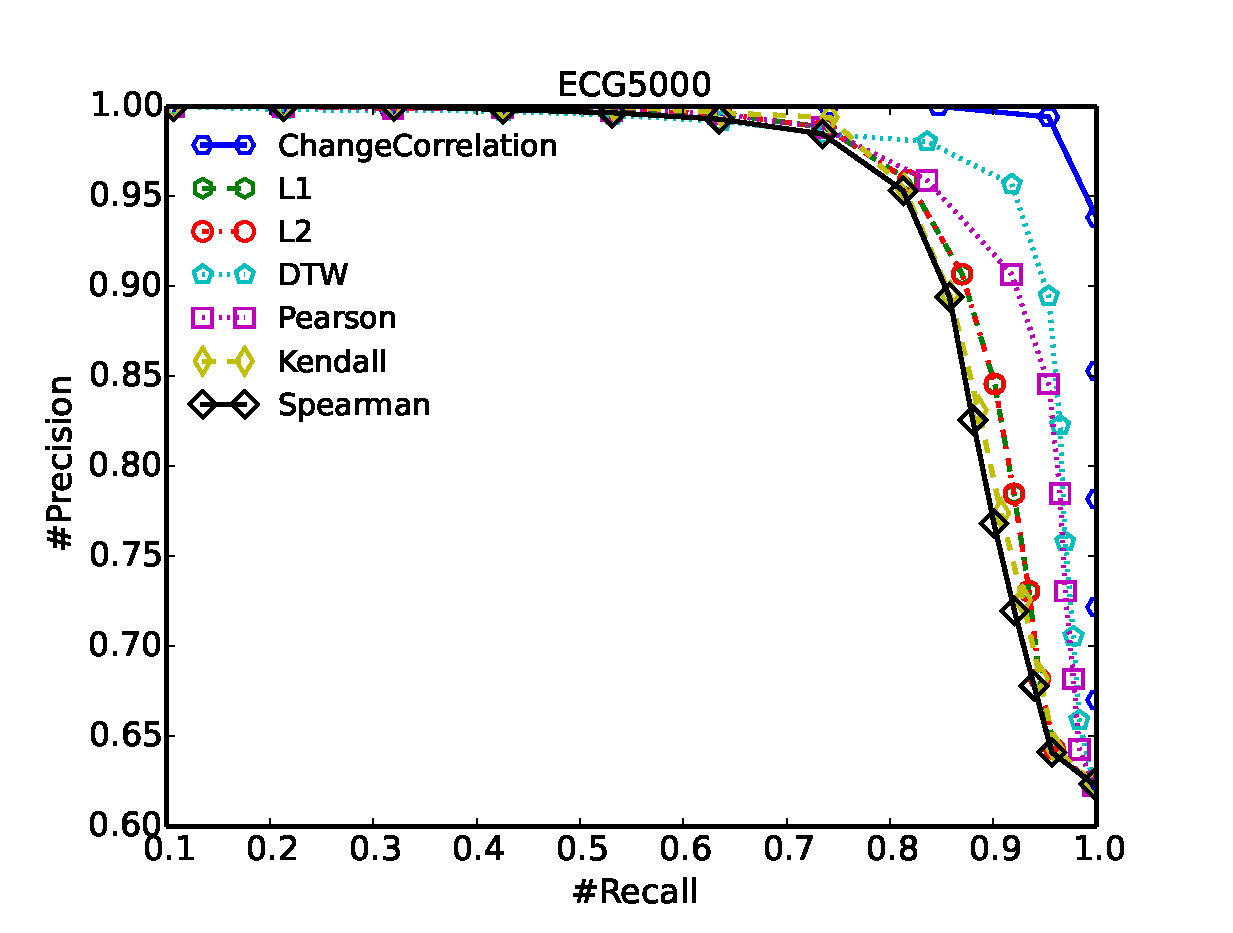
\includegraphics[width=0.45\textwidth]{PRCECG5000.eps}
}\hspace{0.001em}
\subfigure{%
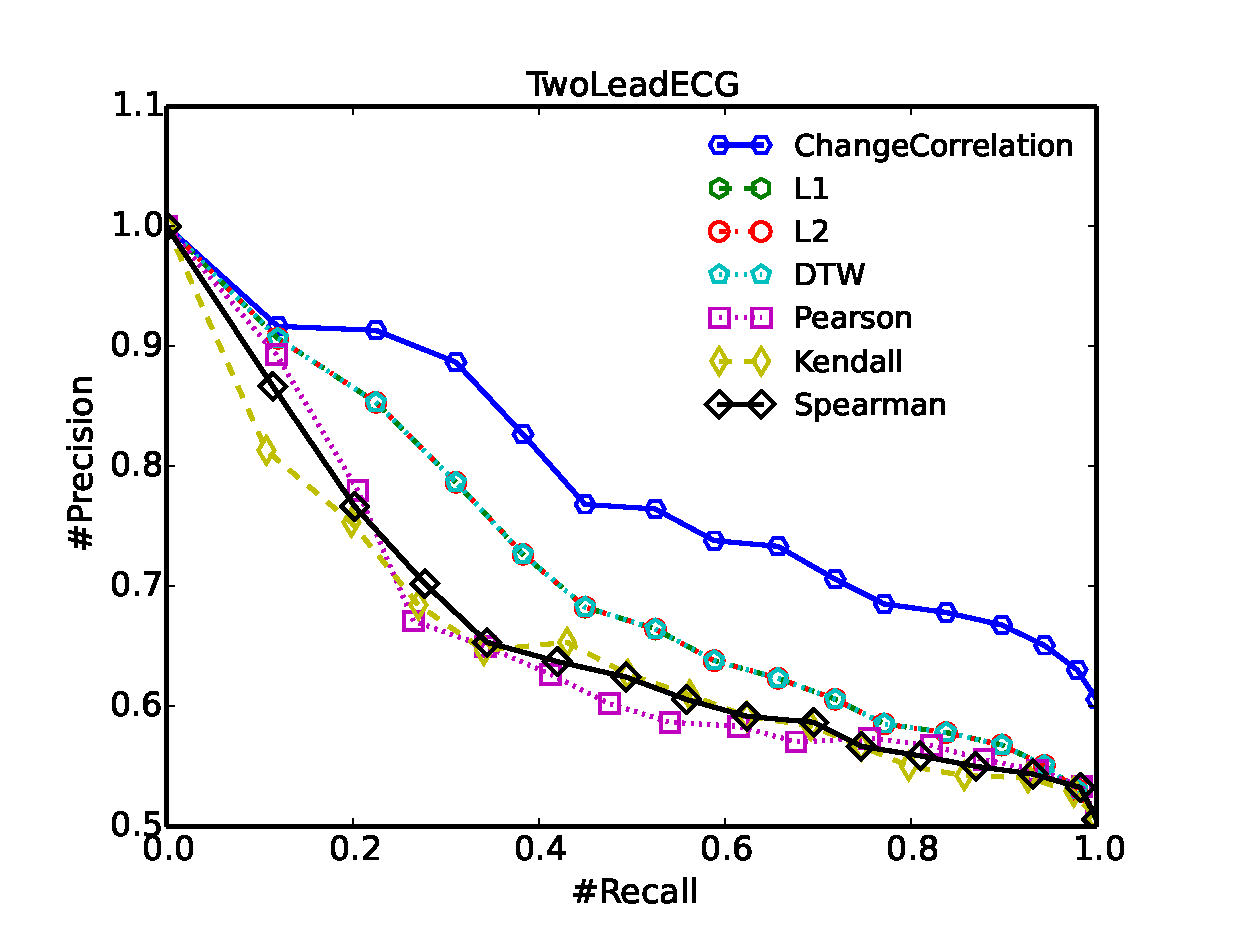
\includegraphics[width=0.45\textwidth]{PRCTwoLeadECG.eps}
}\hspace{0.001em}
\subfigure{%
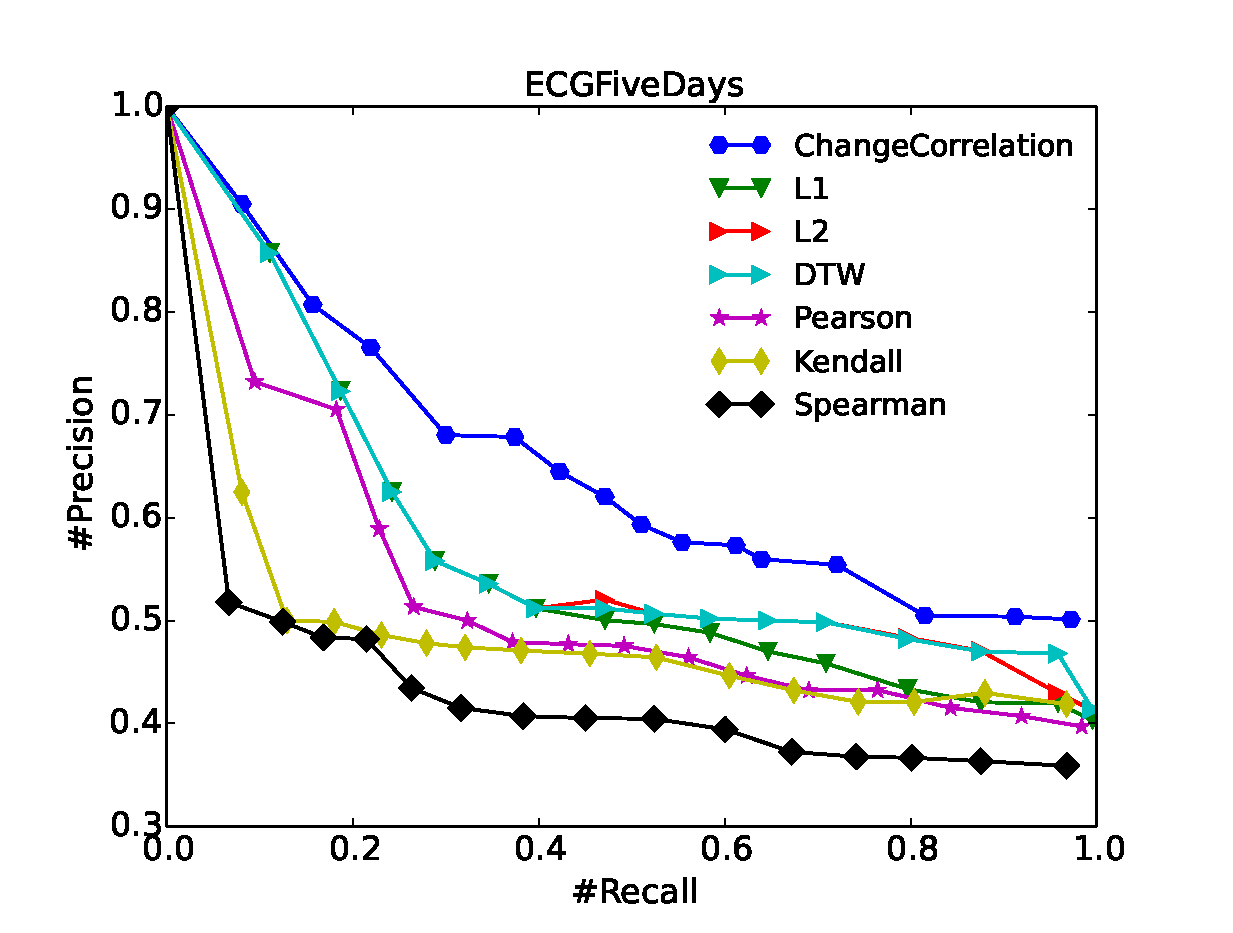
\includegraphics[width=0.45\textwidth]{PRCECGFiveDays.eps}
}\hspace{0.001em}
\caption{Precision Recall Curve (higher is better). We compare Change based correlation coefficient with other methods.}
\label{fig:ECGPRC}
\end{figure*}


\subsubsection{HPC Thread Time Series Data set}

The second real world dataset is from the HPC-tool Kit Dataset. This data set provided by HPCToolkit by analysis High performance computer during running. There are two types of thread in these two data set: main thread and other thread. So, the experiment here is based on the ground truth of two different class of thread.

We also use the Hierarchical Clustering \cite{han2011data} to evaluate the performance as before. 
From Table.\ref{Tab:HPCClus}, we can see that, for the change based correlation can obtain more accuracy results in the two HPC Thread Time series data set compared with both the similarity method and the correlation coefficient. While we can see that DTW method can also get high accuracy, this because in data set, most of the thread in same class often in same state. However, as we said before, in some cases, thread in same class, the state can be different.

The precision recall curve for the HPC Thread TIme Series data is showed in Figure \ref{fig:HPCPRC}. We can clearly see that our proposed Change-based Correlation method gives higher precision recall curves than other similarity and correlation methods. Also, DTW method can get good result too. In addition the results are consistent across datasets. This demonstrate the effectiveness of change-based correlation coefficient and the corresponding LSH search algorithm.

\begin{table}
\caption{Summary of the HPC Time Series Data Set}
\centering

\begin{tabular}{|c|c|c|}
\hline Data Set & \centering Data Size & Time Series Length \\
\hline Single PC & \centering 24 & 4096 \\
\hline MADNESS & \centering 264 & 32768 \\
\hline Environment Simulation & \centering 312 & 16384 \\
\hline
\end{tabular}
\label{Tab:HPCData}
\end{table}

\begin{table*}[t]
\caption{Clustering Performance on Synthetic ECG Data Set From UCR Time Series Archive}
\centering
\renewcommand{\arraystretch}{1.2}
\begin{tabular}{ccccccccc} 
\toprule[2pt] 
%\hline
Dataset & Measure & Proposed & $L1$ & $L2$ & DTW & Pearson & Kendall & Spearman \\
\toprule[1.5pt] 
\multirow{2}*{\centering{Single PC}}
     & Accuracy & $\boldsymbol{.917\pm.011}$ & $.835\pm.068$ & $.815\pm.012$ & $.870\pm.061$ & $.501\pm.140$ & $.527\pm.019$ & $.514\pm.013$ \\
\cline{2-9}
     & NMI & $\boldsymbol{.889\pm.019}$ & $.736\pm.035$ & $.719\pm.023$ & $.860\pm.075$ & $.380\pm.55$ & $.350\pm.015$ & $.349\pm.012$ \\
\toprule[1.2pt] 
\multirow{2}*{\centering{MADNESS}}
     & Accuracy & $\boldsymbol{.938\pm.025}$ & $.927\pm.026$ & $.922\pm.032$ & $.935\pm.012$ & $.457\pm.018$ & $.474\pm.067$ & $.541\pm.067$ \\
\cline{2-9}
     & NMI & $\boldsymbol{.861\pm.030}$ & $.853\pm.062$ & $.857\pm.043$ & $.864\pm.036$ & $.346\pm.084$ & $.404\pm.423$ & $.230\pm.442$ \\
\toprule[1.2pt] 
\multirow{2}*{\centering{Simulation}}
     & Accuracy & $\boldsymbol{.921\pm.021}$ & $.802\pm.026$ & $.420\pm.032$ & $.435\pm.012$ & $.857\pm.018$ & $.464\pm.067$ & $.531\pm.067$ \\
\cline{2-9}
     & NMI & $\boldsymbol{.831\pm.030}$ & $.803\pm.062$ & $.537\pm.043$ & $.504\pm.036$ & $.786\pm.084$ & $.202\pm.423$ & $.330\pm.442$ \\
\toprule[1.2pt] 
\end{tabular}
\label{Tab:HPCClus}
\end{table*}

\begin{figure}[t]
\centering
\subfigure{%
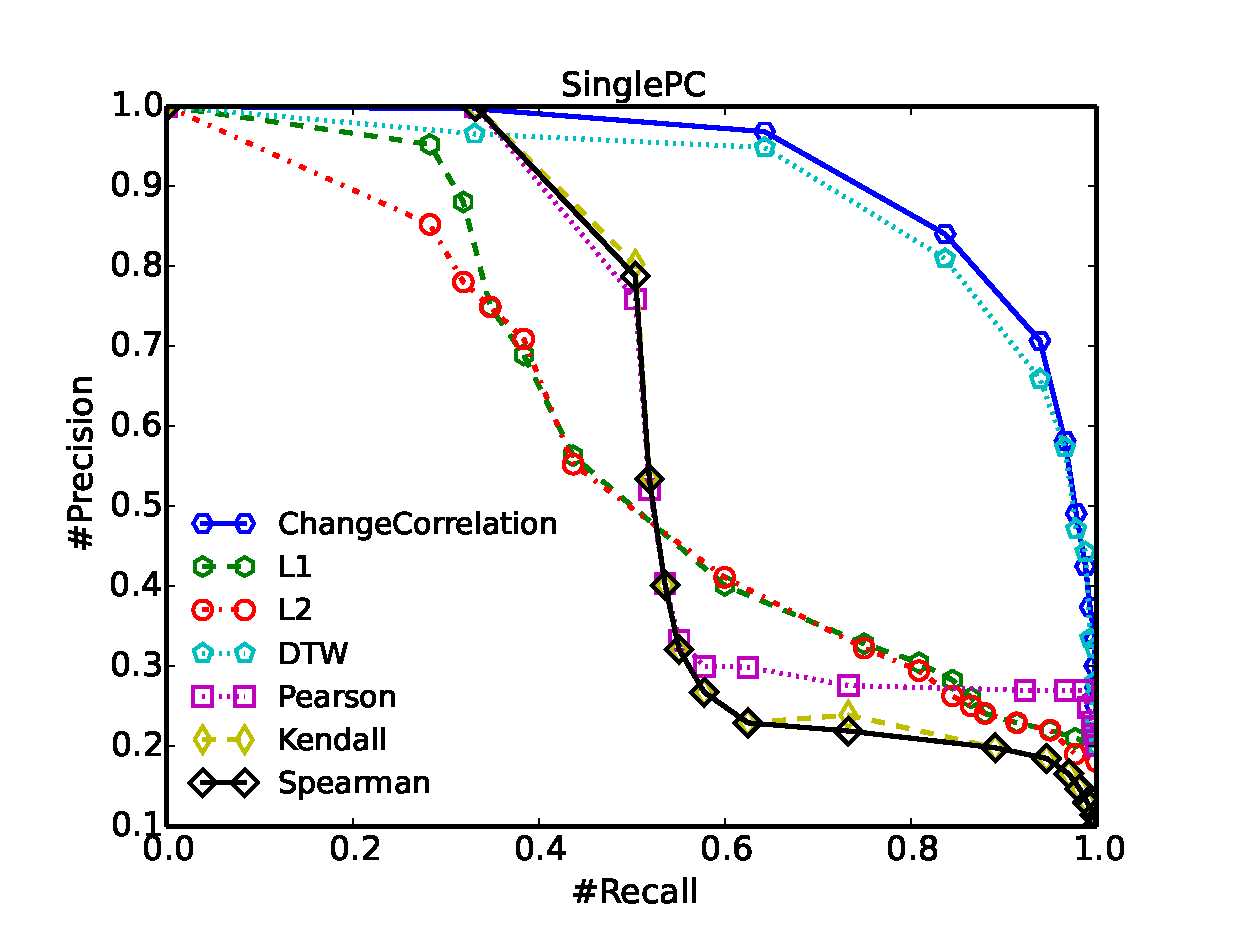
\includegraphics[width=0.45\textwidth]{PRCSinglePC.eps}
}\hspace{0.001em}
\subfigure{%
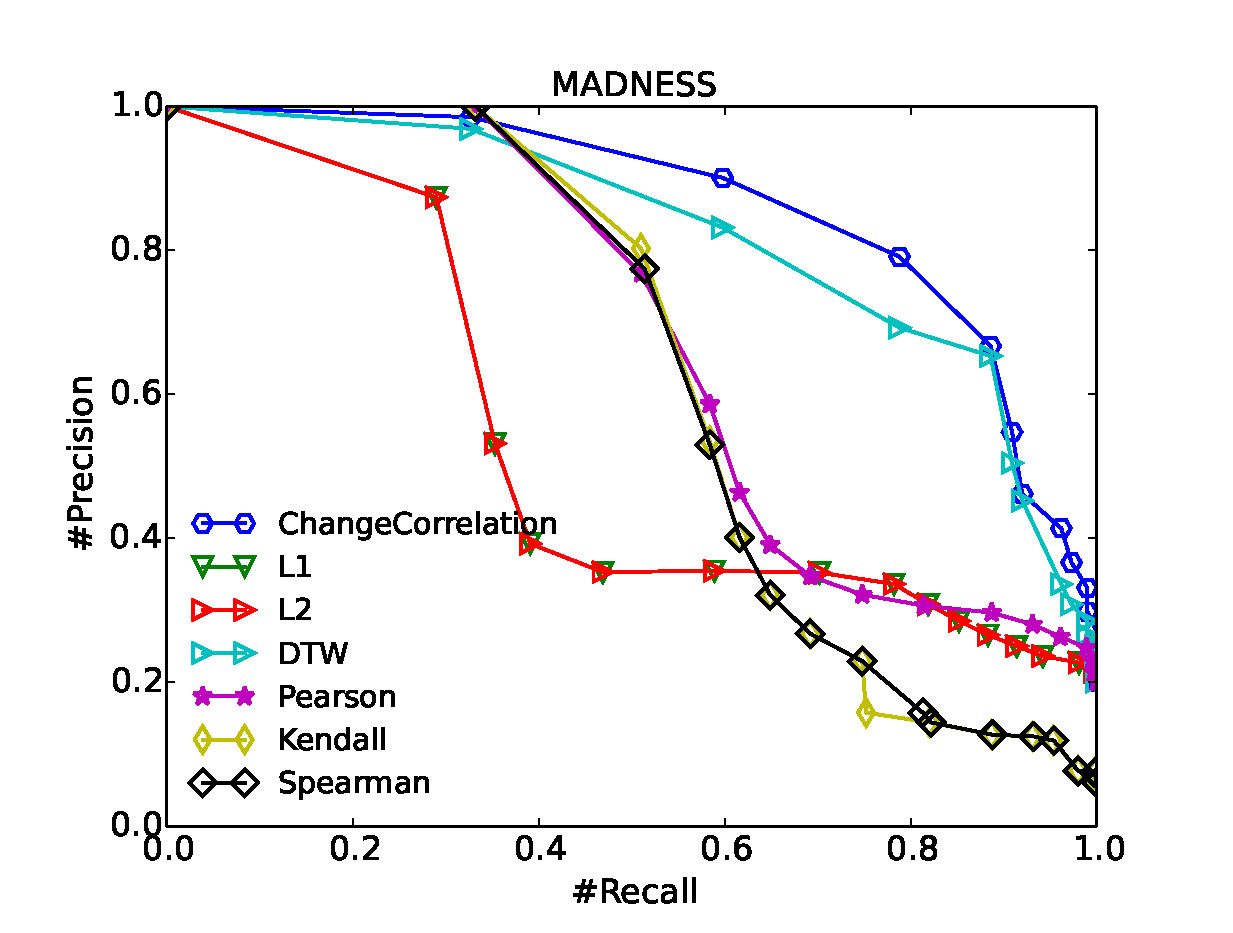
\includegraphics[width=0.45\textwidth]{PRCMADNESS.eps}
}\hspace{0.001em}
\subfigure{%
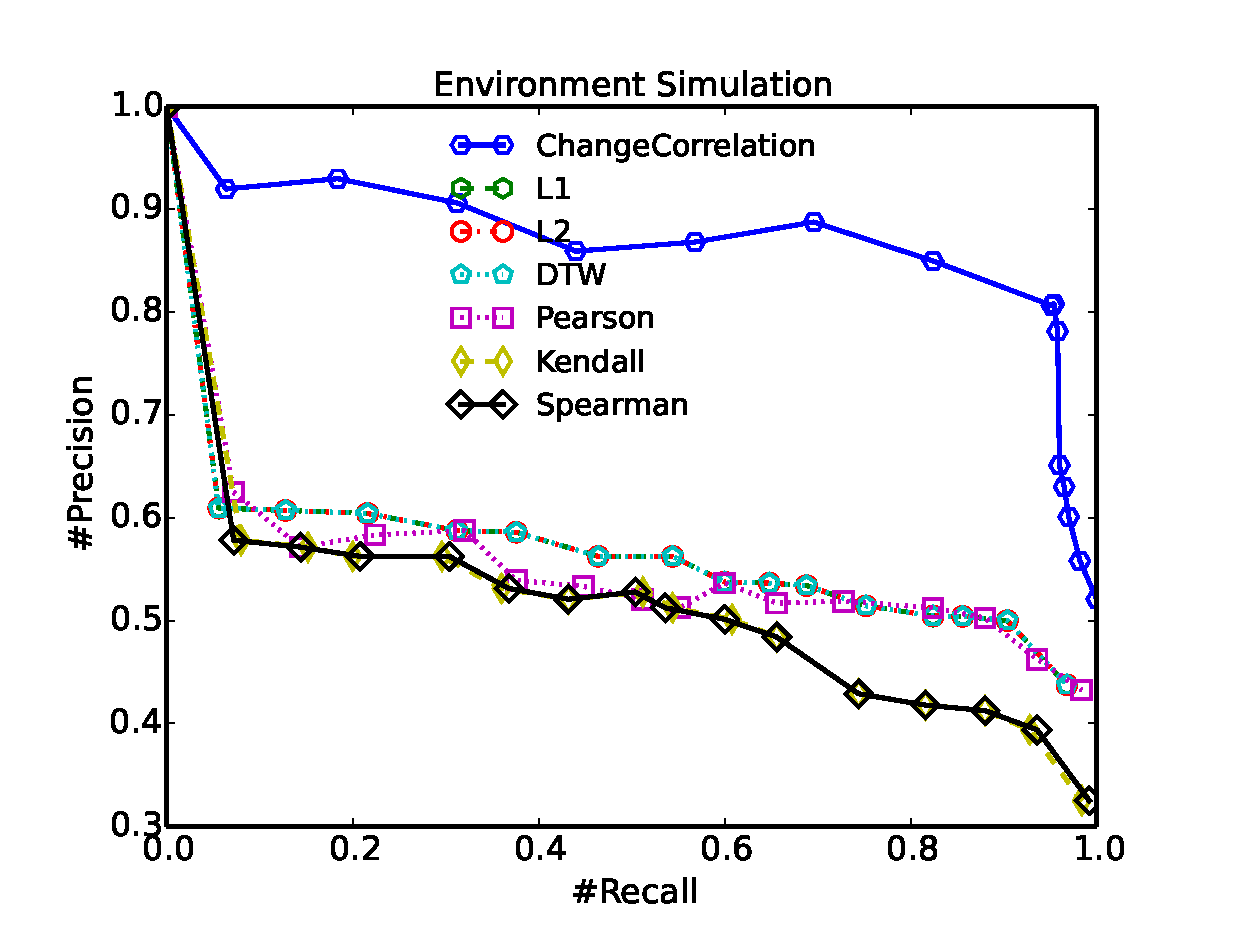
\includegraphics[width=0.45\textwidth]{PRCEnvironment.eps}
}\hspace{0.001em}
\caption{Precision Recall Curve (higher is better). We compare Change based correlation coefficient with other methods.}
\label{fig:HPCPRC}
\end{figure}




